\label{chap:analisi}

\section{Analisi esplorativa}

\begin{definition}
    Una serie di dati è una sequenza ordinata di punti dati, ed esprime la
    dinamica di un certo fenomeno nel tempo. Quando questi dati sono ordinati
    in base al tempo, si parla di una \textbf{serie storica} (o
    \textbf{temporale}).
    Indipendentemente dal criterio utilizzato per ordinarli, i punti dati sono
    registrati seguendo intervalli di tempo equispaziati. Le serie temporali
    possono essere di due tipi: \textbf{univariate}, che coinvolgono una
    singola variabile misurata nel tempo, e \textbf{multivariate}, dove più
    variabili sono misurate contemporaneamente.
\end{definition}

All'interno della tabella \texttt{hj}, che contiene i dati di monitoraggio dei
job eseguiti da HTCondor, ogni riga può essere vista come un punto in una
serie storica multivariata. In altre parole, ciascun job corrisponde a una
serie storica multivariata distinta, dove le variabili rappresentano le
diverse grandezze misurate durante il suo ciclo di vita, come illustrato nella
figura~ \ref{fig:job_time_series}. Sebbene queste serie condividano le stesse
variabili, la durata di ciascun job, e di conseguenza la lunghezza delle
relative serie storiche, cambia.

Come mostrato in figura~\ref{fig:htcondor_sampling}, HTCondor campiona lo
stato di ciascun job ogni tre minuti, ma aggiorna i valori ogni quindici
minuti. Questo significa che ogni serie storica mostra un cambiamento
effettivo nei valori solo ogni cinque campionamenti, risultando in una
sequenza di cinque valori identici che si ripetono fino al prossimo
aggiornamento.

\begin{figure}[p]
    \centering 
    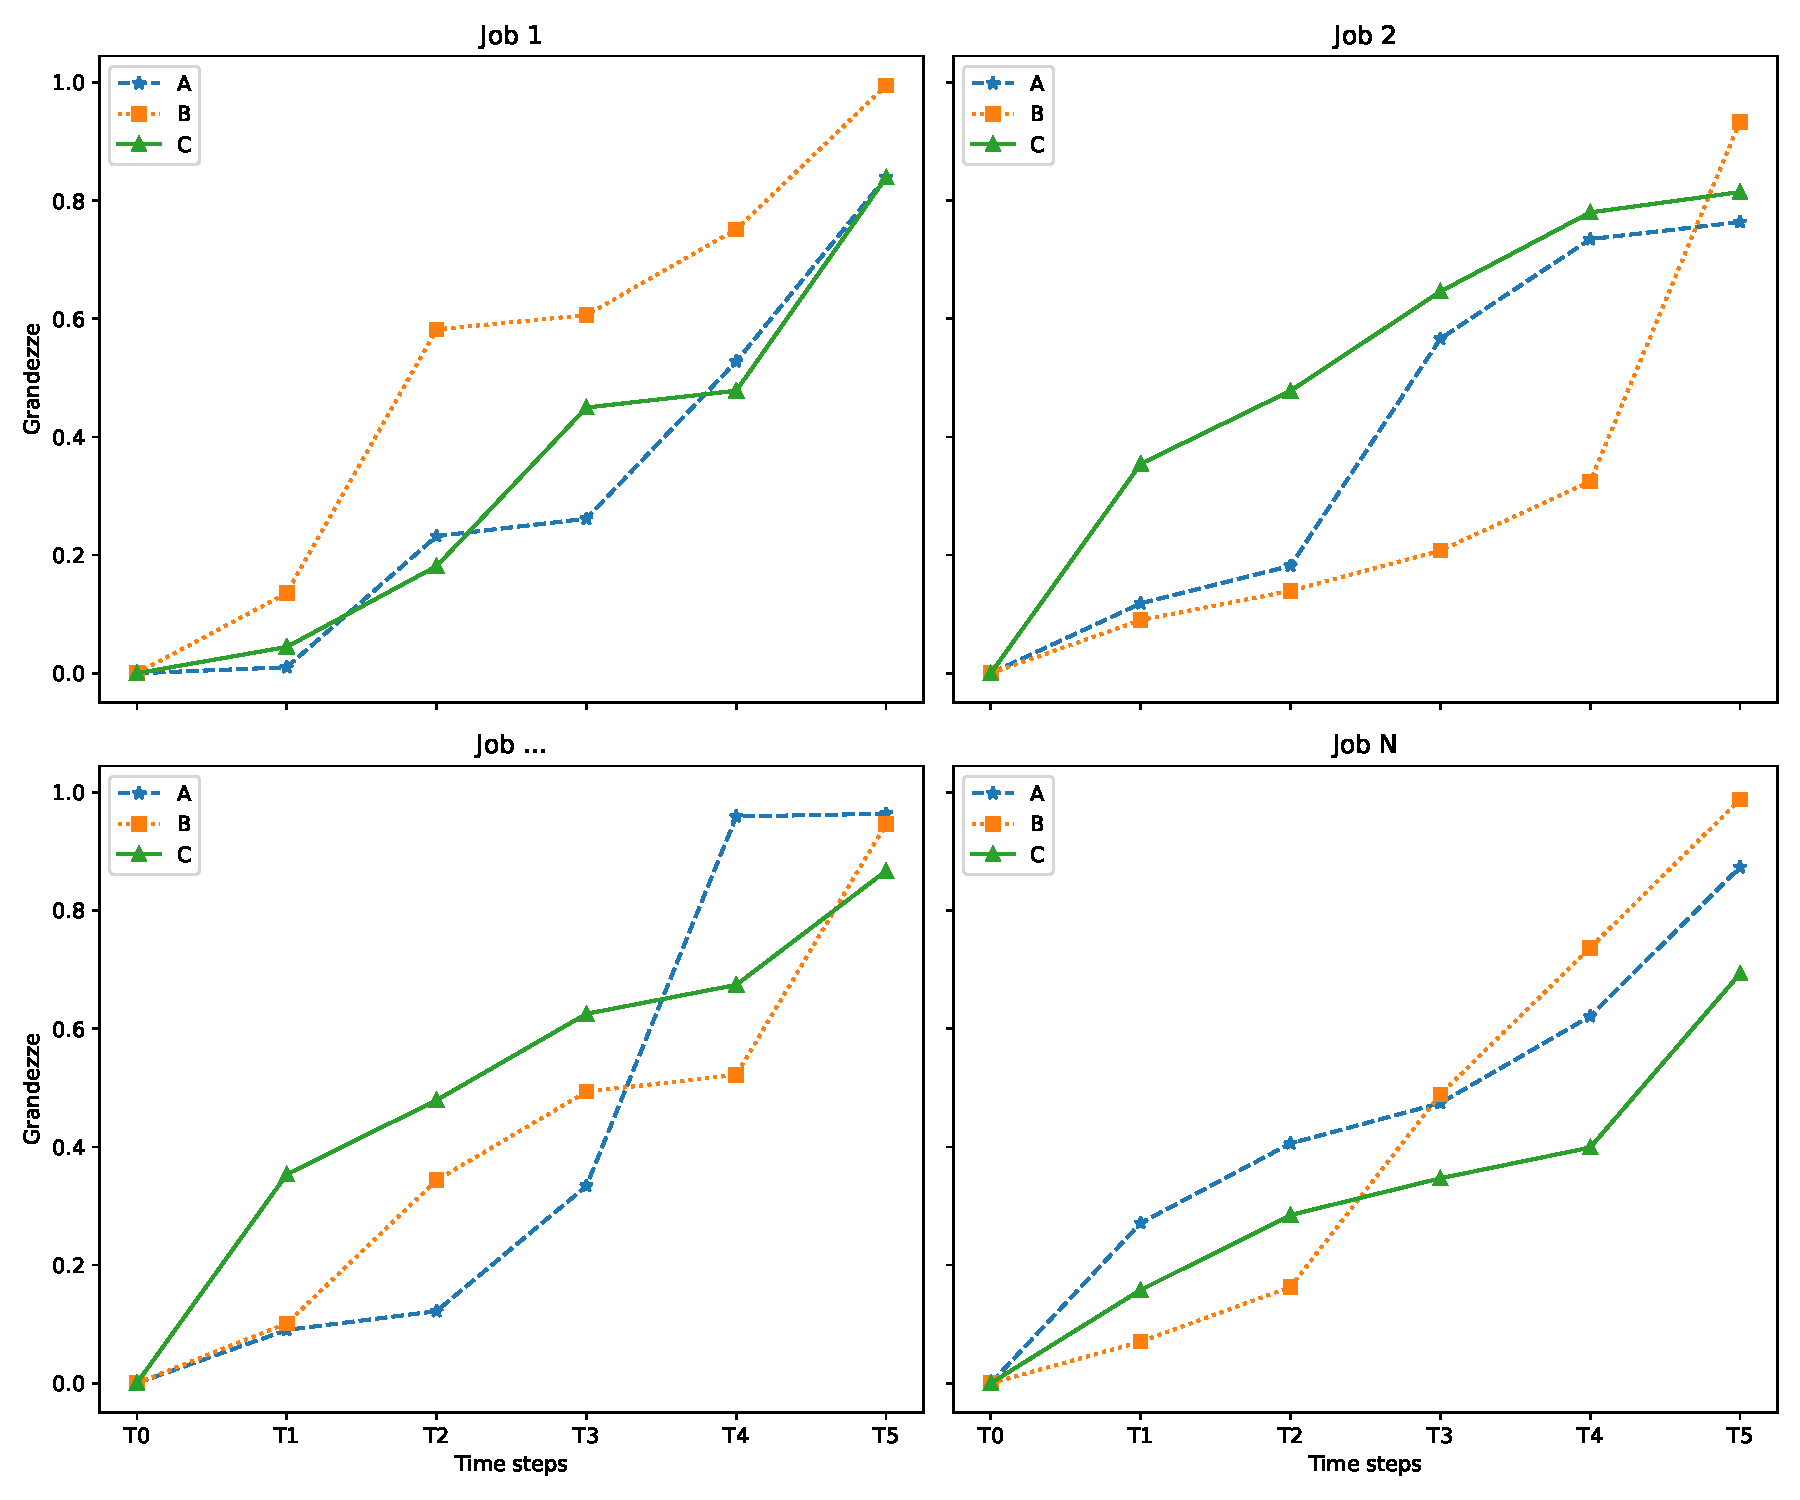
\includegraphics[width=0.95\linewidth]{hj_jobs}
    \caption{\small Rappresentazione di un job come serie storica multivariata}
    \label{fig:job_time_series}
\end{figure}

\begin{figure}[p]
   \centering 
   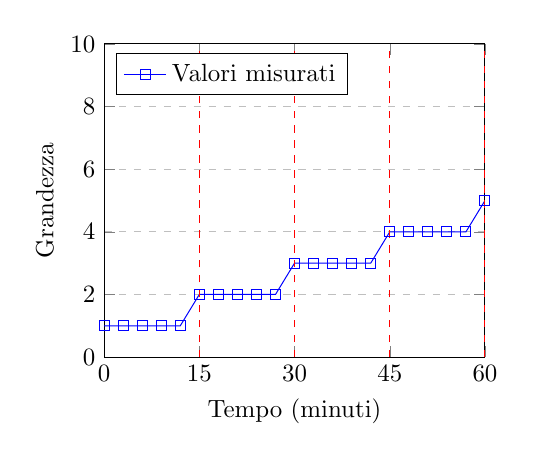
\begin{tikzpicture}[scale=0.9]
       \begin{axis}[
           xlabel={Tempo (minuti)},
           ylabel={Grandezza},
           xmin=0, xmax=60,
           ymin=0, ymax=10,
           xtick={0, 15, 30, 45, 60},
           ytick={0,2,4,6,8,10},
           legend pos=north west,
           ymajorgrids=true,
           grid style=dashed,
           height=6cm
           ]

           % serie storica
           \addplot[color=blue, mark=square]
           coordinates {
               (0,1) (3,1) (6,1) (9,1) (12,1) 
               (15,2) (18,2) (21,2) (24,2) (27,2) 
               (30,3) (33,3) (36,3) (39,3) (42,3) 
               (45,4) (48,4) (51,4) (54,4) (57,4) (60,5)
           };
           \addlegendentry{Valori misurati}

           \draw[dashed, red] (15,0) -- (15,10);
           \draw[dashed, red] (30,0) -- (30,10);
           \draw[dashed, red] (45,0) -- (45,10);
           \draw[dashed, red] (60,0) -- (60,10);
       \end{axis}
   \end{tikzpicture}
   \caption{\small Frequenza di campionamento e aggiornamento dei job in HTCondor}
   \label{fig:htcondor_sampling}
\end{figure}

Per quanto riguarda l'aggiornamento dei valori, HTCondor aggiorna un nuovo
dato all'interno della serie storica solo quando il valore rilevato supera il
precedente massimo. Di conseguenza, ciascuna serie storica può essere vista
come una funzione monotona non decrescente, in cui ogni nuovo valore
registrato è maggiore o uguale al precedente.

La durata dei job varia considerevolmente, come mostrato dalla distribuzione
del numero di job rispetto alla loro durata in giorni, illustrata nella
figura~\ref{fig:job_duration_days}. Vi è una predominanza di job di breve
durata, con un calo esponenziale del numero di job al crescere della durata.

\begin{figure}[!h]
   \centering
   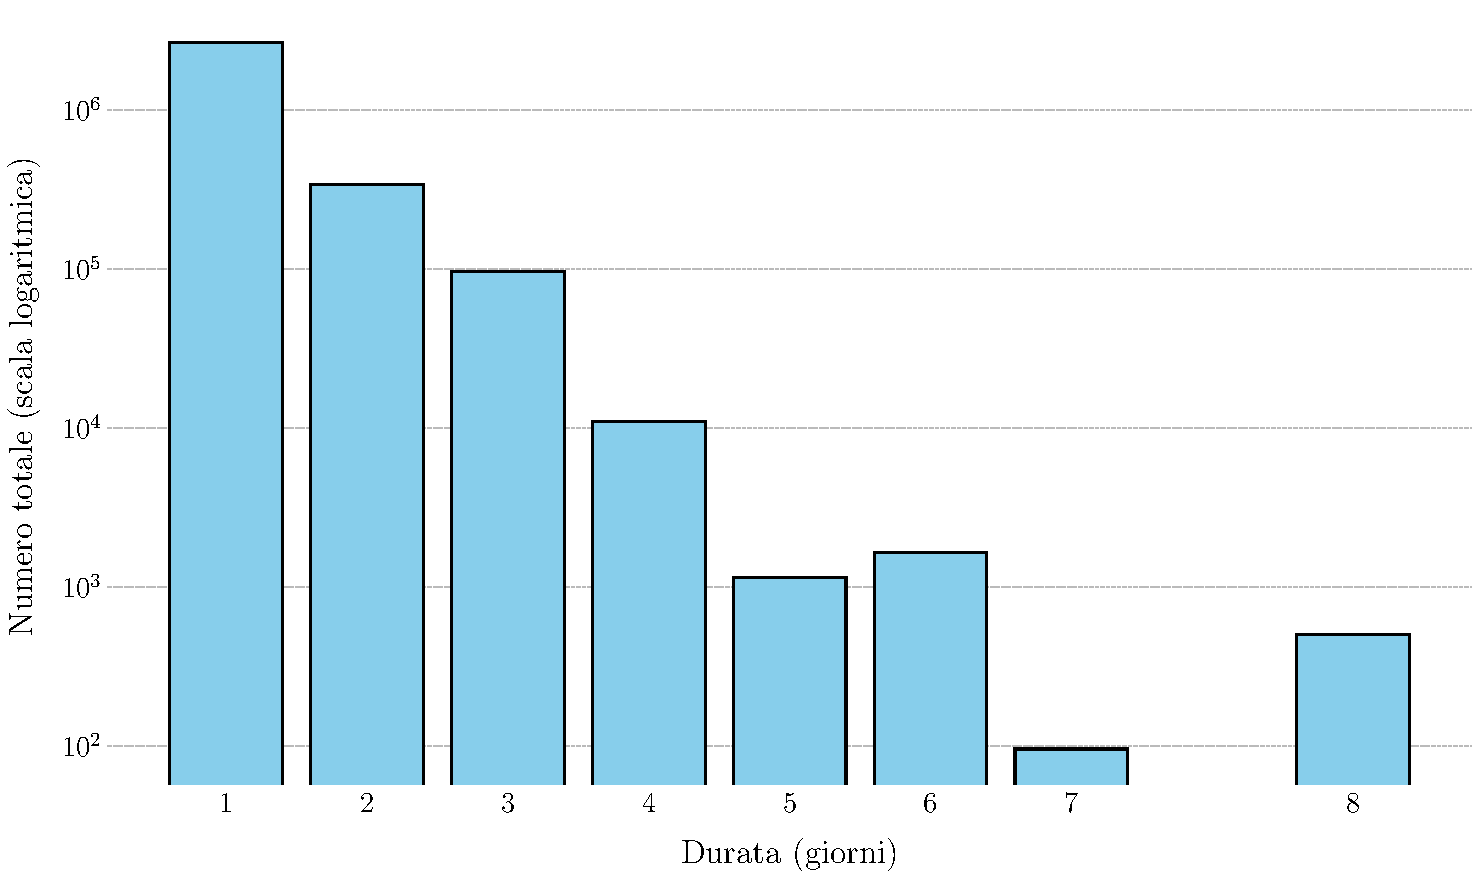
\includegraphics[width=0.85\linewidth]{job_duration_days}
   \caption{}
   \label{fig:job_duration_days}
\end{figure}
% i gruppi hanno distribuzioni diverse

Raggruppando i job in base alla loro durata in fasce orarie fino a un massimo
di 48 ore e aggregando tutti quelli che superano tale soglia, è possibile
esaminare il numero totale dei job, la frequenza dei loro fallimenti e il
cumulativo della loro durata per ciascuna delle prime quarantotto ore, così
come per quelli più lunghi. Come evidenziato nella
figura~\ref{fig:njobs_and_rt_perhour}, i job che durano meno di un'ora sono
particolarmente numerosi e presentano un elevato tasso di fallimento.
Nonostante ciò, il tempo speso sulle risorse di calcolo è pressoché
trascurabile se confrontato con il tempo impiegato dai job di durata
superiore.

\begin{figure}[p]
    \centering
    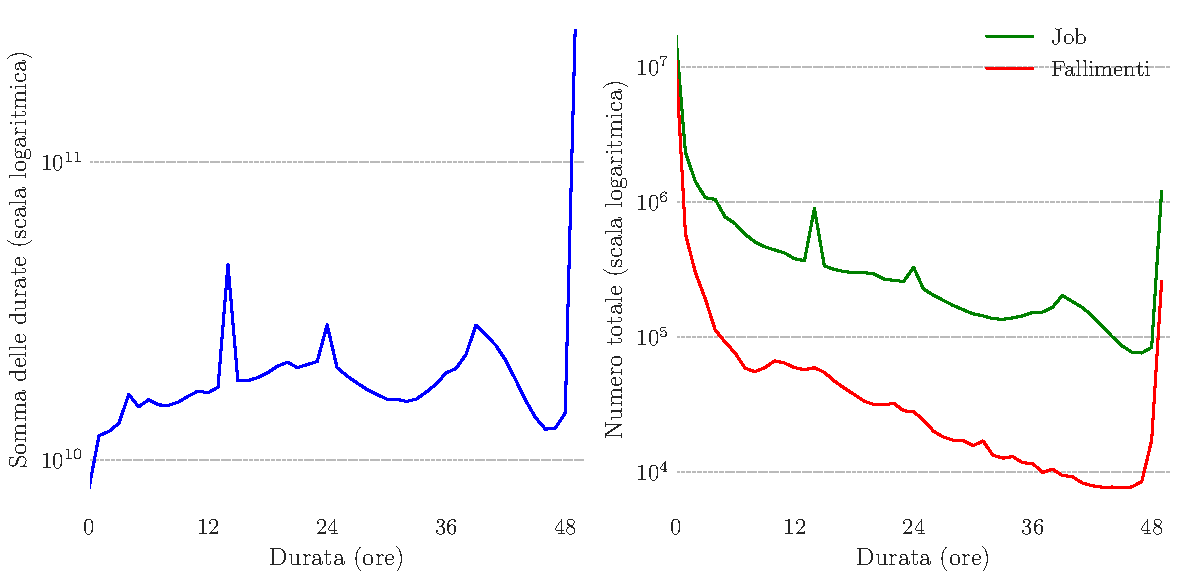
\includegraphics[width=\linewidth]{njobs_and_rt_perhour}
    \caption{\small A sinistra, durata cumulativa dei job; a destra, numero
    totale di job e relativi fallimenti per ogni fascia oraria fino a 48 ore,
mostrati su scala logaritmica}
    \label{fig:njobs_and_rt_perhour}
\end{figure}

Inoltre, se ci focalizziamo sulla prima ora e suddividiamo i job in intervalli
di cinque minuti, possiamo notare che molti di essi hanno una durata inferiore
ai cinque minuti, come si può vedere nella figura~\ref{fig:jobs_firsthour}.
Questo suggerisce che questi job potrebbero essere considerati come semplici
tentativi; in altre parole, sono job che, per vari motivi, non trovano le
condizioni necessarie per proseguire nella loro esecuzioni e quindi
falliscono.

\begin{figure}[p]
   \centering
   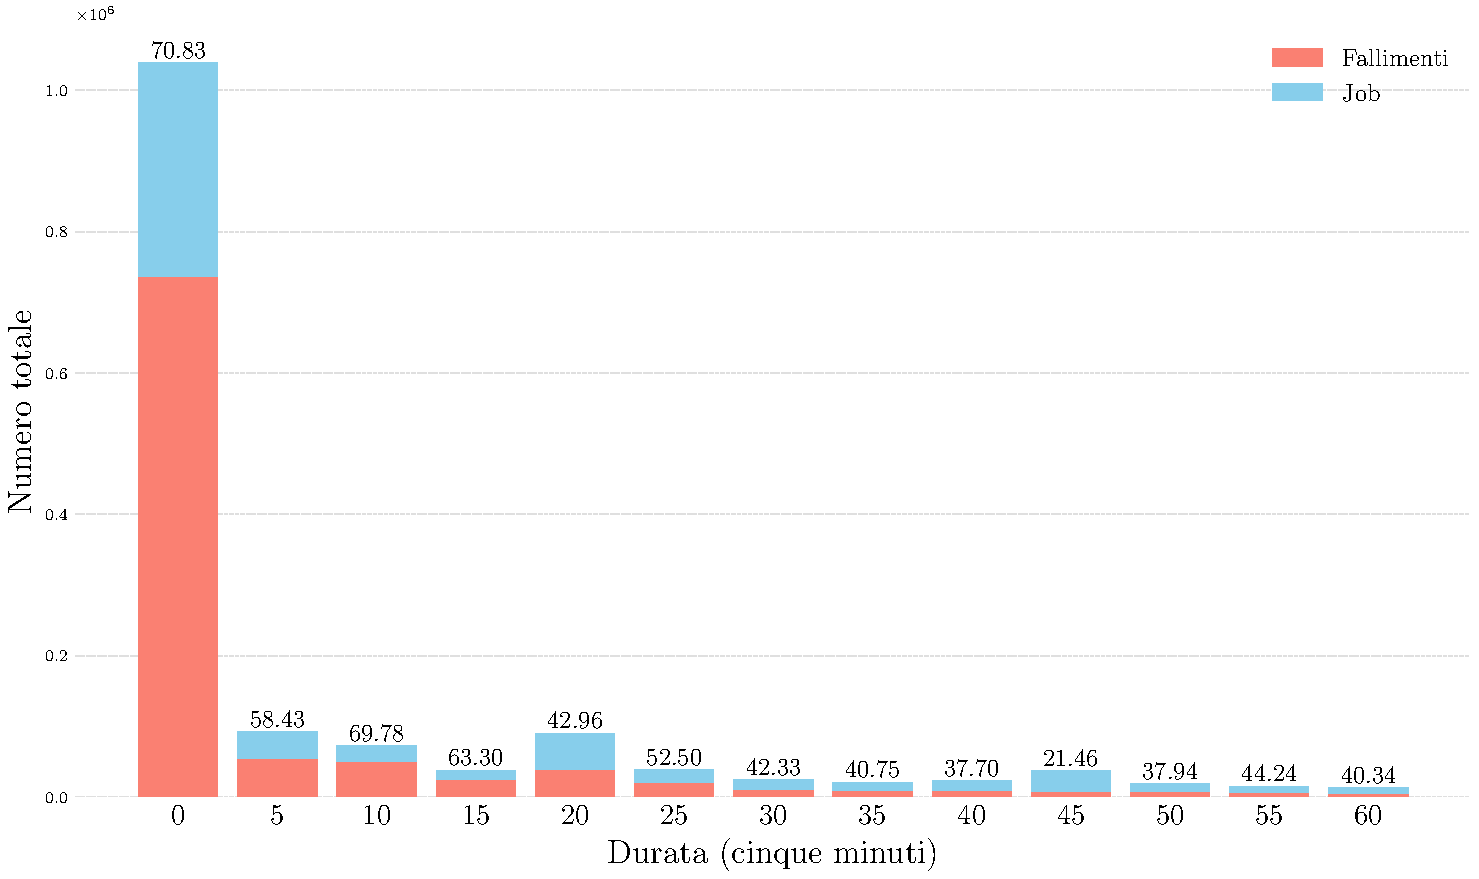
\includegraphics[width=\linewidth]{njobs_firsthour_perfiveminutes}
   \caption{\small Distribuzione dei job nella prima ora, suddivisi in intervalli di
   cinque minuti}
   \label{fig:jobs_firsthour}
\end{figure}

In aggiunta, secondo quanto riportato nella
tabella~\ref{table:pending_jobs_removed}, un significativo 11\% dei job viene
terminato ancor prima di raggiungere la fase di esecuzione. Questi job, non
giungendo alla fase di esecuzione, non effettuano alcun calcolo, il che
sottolinea la presenza di un elevato numero di tentativi che risultano
irrilevanti in termini di calcolo.

\begin{table}[!h]
    \caption{Percentuale di job in attesa rimossi senza aver effettuato alcun
    calcolo su un host fisico}
    \centering
    \begin{tabular}{ccc}
        \toprule
        \textbf{Job in attesa rimossi} & \textbf{Job eseguiti totali} &
        \textbf{Percentuale} \\
        \midrule
        402,663 & 3,589,280 & 11.22 \\
        \bottomrule
    \end{tabular}
    \label{table:pending_jobs_removed}
\end{table}

Pertanto, alla luce di queste considerazioni, nasce la seguente idea:
\begin{quote}
    \emph{Predire il fallimento di un job di lunga durata è nettamente più
    importante rispetto alla previsione del fallimento di un job di breve durata}.
\end{quote}



\section{Job Zombie Prediction}



% chi sono i job zombie 
% timeout grid 3 giorni
% timeout local 7 giorni 

% tempo di timeout code LHC e code non LHC

% le code LHC sono quelle caratterizzate maggiormente da job zombie 

% tempo perso per job zombie 

\begin{table}[!h]
    \centering
    \caption{Descrizione dei dati di esecuzione dei job}
    \begin{tabular}{lllll}
        \toprule
        \textbf{Gruppo} & \textbf{Job zombie} & \textbf{Job totali} &
        \textbf{perc\_time\_lost} & \textbf{Giorni persi} \\
        \midrule
        lhcb & 192 & 262251 & 0.073212 & 576 \\
        juno & 151 & 10137 & 1.489593 & 453 \\
        atlas & 45 & 270086 & 0.016661 & 135 \\
        lhcf & 8 & 1594 & 0.501882 & 24 \\
        belle & 2 & 42087 & 0.004752 & 6 \\
        \bottomrule
    \end{tabular}
    \label{table:job_zombie_timelost}
\end{table}

% sbilanciamento delle classi

% sono separabili questi job dai job normali e su che base

% Un autoencoder, in particolare se profondo e ben regolarizzato, p

Per stabilire se l'applicazione di tecniche di Machine Learning è fattibile
nel rilevare i cosiddetti ``job zombie'', è essenziale verificare
preliminarmente la presenza di cluster ben definiti all'interno del dataset.
L'obiettivo sarebbe quello di distinguere con precisione questi job anomali
dagli altri. 

L'algoritmo t-Distribuited Stochastic Neighbor Embedding (t-SNE) consente di
ridurre la dimensionalità dei dati preservando la vicinanza tra i punti simili
e distanziando quelli dissimili \cite{geron2019}. Passando da uno spazio ad alta
dimensionalità a uno spazio bidimensionale o tridimensionale è possibile la
visualizzazione dei dati attraverso uno scatterplot.

% autoencoder + t-SNE
% possono essere difficili da catturare con metodi lineari come PCA prima
% dell'applicazione di t-SNE.


\section{Preparazione dei dati per il task di ML}
\subsection{Trasformazione delle serie storiche multivariate multiple}

% dobbiamo convertire le serie storiche in un tipo di dati strutturato,
% tabellare, utilizzabile dai modelli di Machine Learning

% padding e truncate delle serie storiche 

% avg pooling

% tabular transformation

% tensor transformation

\subsection{Creazione delle feature}
% jobid e idx

% jobid e idx sono creati dal Submit Node al "concepimento" del job (es.
% 'sn-01', 'ce03-htc', ...). I S.N. sono indipendenti tra loro per cui in linea
% di principio possono esistere due job diversi con (jobid,idx) uguale (in tal
% caso vengono da S.N. diversi)%

% job work type

% job type

% one hot encoding 

% non verranno considerati i jobs con runtime <
% 1h, poichè non rilevanti per il sistema.

\subsection{Labeling dei dati}
\subsection{Tecniche di bilanciamento dei dati}

% undersample

% oversample

% class weighting in loss function

% metriche
